\documentclass[sigconf]{acmart}

\usepackage{xspace}
\usepackage{graphics}
\usepackage[T1]{fontenc}
\usepackage{times}
\usepackage{color}
\usepackage{booktabs}
\usepackage{textcomp}
\usepackage{microtype}
\usepackage{ccicons}
\usepackage{todonotes}
\usepackage{amsthm}
\usepackage{amsmath}
\usepackage{subcaption}
\usepackage{hyperref}
\usepackage{url}
\usepackage{relsize}
\usepackage{caption}
\usepackage{soul}
\usepackage[normalem]{ulem}
\newtheorem{example}{Example}
\hypersetup{
  colorlinks,
  urlcolor=blue}
\renewcommand*{\UrlFont}{\ttfamily\smaller\relax}

\newcommand{\stepCounter}[1]{{\Large\textcircled{{\small#1}}}}

\AtBeginDocument{%
  \providecommand\BibTeX{{%
    \normalfont B\kern-0.5em{\scshape i\kern-0.25em b}\kern-0.8em\TeX}}%
  \raggedbottom
}
\setcopyright{acmcopyright}
\copyrightyear{2024}
\acmYear{2024}
\acmDOI{XXXXXXX.XXXXXXX}
\acmConference[SIGMOD '24]{International Conference on Management of Data}{June 09--15, 2024}{Santiago, Chile}
\acmPrice{15.00}
\acmISBN{978-1-4503-XXXX-X/18/06}

\setcopyright{none}
\renewcommand\footnotetextcopyrightpermission[1]{}
\settopmatter{printacmref=false}
\acmDOI{}
\acmConference[]{}{}{}
\acmBooktitle{}
\acmISBN{}
\date{}

% Packages needed by the literature-review content
\usepackage{array}
\usepackage{balance}
\usepackage{capt-of}
\usepackage{dblfloatfix}
\usepackage{float}
\usepackage{forest}
\usepackage{makecell}
\usepackage{multirow}
\usepackage{placeins}
\usepackage{ragged2e}
\usepackage{tabularx}
\usepackage{tikz}
\usepackage{xcolor}
\usetikzlibrary{positioning,calc,arrows.meta}

% --- floats (two-column) ---
\setcounter{topnumber}{2}
\setcounter{dbltopnumber}{2}
\renewcommand{\topfraction}{0.9}
\renewcommand{\dbltopfraction}{0.9}
\renewcommand{\textfraction}{0.07}
\renewcommand{\floatpagefraction}{0.85}
\renewcommand{\dblfloatpagefraction}{0.85}

\setlength{\textfloatsep}{8pt plus 2pt minus 2pt}
\setlength{\dbltextfloatsep}{8pt plus 2pt minus 2pt}
\setlength{\floatsep}{6pt plus 2pt minus 2pt}
\setlength{\dblfloatsep}{6pt plus 2pt minus 2pt}
\setlength{\intextsep}{6pt plus 2pt minus 2pt}

% Custom X-like column
\newcolumntype{Y}{>{\RaggedRight\arraybackslash}X}

% One table formatting macro used everywhere
\newcommand{\tbl}{%
  \scriptsize
  \setlength{\tabcolsep}{4pt}%
  \renewcommand{\arraystretch}{1.12}%
}

\begin{document}
\pagestyle{plain}

% ======================
% Title + Authors
% ======================
\title[Survey of Data Discovery to Integration in Data Lakes]%
{From Data Discovery to Analytics-Ready Data:\\A Survey of Search, Preparation, and Integration in Data Lakes}

\author{Sumaiya Azad}
\affiliation{%
  \institution{University of Utah}
  \city{Salt Lake City}
  \state{Utah}
  \country{USA}}
\email{sumaiya.azad@utah.edu}

\renewcommand{\shortauthors}{Azad}


% ======================
% Abstract
% ======================

\begin{abstract}
Organizations collect many kinds of data in data lakes. Before analysts can query those data or build dashboards from them, they must find relevant sources, clean and organize them, and combine information across sources.

I review 47 methods published from 2022 to 2025 and organize them into three phases: \emph{Discovery \& Search}, \emph{Preparation \& Wrangling}, and \emph{Integration \& Matching}. For each phase, I describe common tasks, system designs, and evaluation practices. I close with open challenges in end-to-end evaluation, keeping results up to date as data changes, and reliable use of language models for data tasks.
\end{abstract}

% ======================
% CCS Concepts (single block)
% ======================
\begin{CCSXML}
<ccs2012>
 <concept>
  <concept_id>10002951.10003260</concept_id>
  <concept_desc>Information systems~Information integration</concept_desc>
  <concept_significance>500</concept_significance>
 </concept>
 <concept>
  <concept_id>10002951.10003260.10003300</concept_id>
  <concept_desc>Information systems~Data cleaning</concept_desc>
  <concept_significance>500</concept_significance>
 </concept>
 <concept>
  <concept_id>10002951.10003260.10003309</concept_id>
  <concept_desc>Information systems~Data exchange</concept_desc>
  <concept_significance>300</concept_significance>
 </concept>
 <concept>
  <concept_id>10002951.10003260.10003305</concept_id>
  <concept_desc>Information systems~Data mining</concept_desc>
  <concept_significance>300</concept_significance>
 </concept>
 <concept>
  <concept_id>10002951.10003260.10003310</concept_id>
  <concept_desc>Information systems~Data retrieval</concept_desc>
  <concept_significance>300</concept_significance>
 </concept>
</ccs2012>
\end{CCSXML}

\ccsdesc[500]{Information systems~Information integration}
\ccsdesc[500]{Information systems~Data cleaning}
\ccsdesc[300]{Information systems~Data exchange}
\ccsdesc[300]{Information systems~Data mining}
\ccsdesc[300]{Information systems~Data retrieval}


\keywords{data lakes, dataset discovery, table search, join discovery, union discovery, data preparation, data wrangling, data cleaning, schema matching, entity resolution, data integration, analytics-ready data}


\maketitle

% ==========================================================
\section{Introduction}
Data lakes~\cite{10.1145/3555041.3589409,10.14778/3750601.3750694} store many kinds of data together---spreadsheet-like tables, semi-structured files such as JSON or XML, server logs, and fields pulled from documents---without requiring one fixed column layout, or \emph{schema}, at load time.
Loading data is easy, but using it later is hard.
Before analysts can run queries, build dashboards, or train models, they must (1)~find the right data, (2)~clean and organize it, and (3)~combine it from multiple sources.

\paragraph{Scope and terminology.}
\emph{Discovery} means finding relevant tables or columns, including \emph{join} search~\cite{10.1145/3555041.3589409} (tables sharing a key column) and \emph{union} search~\cite{10.14778/3750601.3750694} (tables with compatible columns). \emph{Preparation} means cleaning errors, transforming values, and organizing raw data into usable tables or reusable workflows. \emph{Integration} means lining up columns across sources and producing a merged output; \emph{entity resolution (ER)} is the special case of deciding whether two records describe the same real-world thing. I use \emph{analytics-ready data} to mean data that is clean and structured enough for reports, statistics, or machine learning.

Two trends make this pipeline harder: (1)~modern lakes are large and weakly documented; (2)~embedding-based and language-model-based methods now appear in discovery~\cite{10.14778/3659437.3659461}, preparation~\cite{10.14778/3611540.3611624}, and integration~\cite{10.14778/3742728.3742757}, raising concerns about cost, reliability, and privacy.

This survey follows the full path from raw lake data to analytics-ready outputs in three phases:
(1) \emph{Discovery \& Search} finds relevant tables and ranks candidates that could be joined or unioned;
(2) \emph{Preparation \& Wrangling} cleans, restructures, and transforms selected data into usable tables or reusable automated workflows; and
(3) \emph{Integration \& Matching} lines up columns and records across sources to produce a single merged dataset.
I describe my six-step process for selecting and organizing methods in Section~\ref{sec:methodology}.

My main focus is the connection among these three phases. Instead of treating discovery, preparation, and integration as separate tasks, I study them as one pipeline where each stage feeds the next.

\paragraph{Contributions.}
\begin{itemize}
  \item I review methods from three top database venues (SIGMOD, PVLDB, and ICDE) using a clear process for selecting and categorizing them (Section~\ref{sec:methodology}).
  \item I propose a taxonomy that groups methods by what they produce---ranked candidate lists, cleaned tables, automated workflows, column matches, or merged datasets---spanning discovery, preparation, and integration (Section~\ref{sec:taxonomy-classes}).
  \item I summarize the tasks, system designs, and evaluation practices in each phase, including trade-offs between effectiveness, cost, and the need for human oversight (Section~\ref{sec:pubs-by-phase}).
  \item I identify open problems, including pipeline-level evaluation, keeping results up to date as data changes, reliable use of language models, fairness and privacy constraints, and the need for shared test collections (Section~\ref{sec:discussion-challenges}).
\end{itemize}


% ==========================================================
\section{Related Work}
\label{sec:related}
Earlier surveys cover \emph{discovery} in data lakes in depth, including keyword search, join discovery, and union discovery~\cite{10.1145/3555041.3589409}, as well as indexing and benchmarking~\cite{10.14778/3750601.3750694}. These surveys clearly define the main discovery tasks and compare systems in detail.

Other work studies individual tasks such as \emph{data cleaning}~\cite{10.14778/3675034.3675051}, \emph{schema matching}~\cite{10.14778/3742728.3742757}, and \emph{entity resolution}~\cite{10.1145/3588722}. I instead focus on recent work across the three phases, which lets me capture language-model-based methods, newer system designs, and emerging concerns such as cost, reliability, fairness, and privacy.


% ==========================================================
\section{Methodology}
\label{sec:methodology}
This section explains how I found, selected, and organized the methods in this survey, with enough detail to reproduce the search and check inclusion decisions.

\paragraph{Step 1: Research questions.}
For each method I ask four questions: (i)~which phase does it target (discovery, preparation, or integration)? (ii)~what does it mainly produce (for example, a ranked list, a cleaned table, or a merged dataset)? (iii)~what technique does it use? and (iv)~how is it evaluated (which datasets, which metrics, and whether cost is reported)?

\paragraph{Step 2: Search terms.}
I search using the query \texttt{"data lake" AND (S1 OR S2 OR S3 OR S4)}, where S1 through S4 are groups of task-related keywords listed in Table~\ref{tab:search-strings}.


% ---------- Table: Search terms ----------
\begin{table}[!htbp]
\caption{Search term groups used for queries over data lakes.}
\label{tab:search-strings}
\centering
\tbl
\begin{tabularx}{\columnwidth}{@{}p{8mm}X@{}}
\toprule
\textbf{ID} & \textbf{Query family (examples of task keywords)} \\
\midrule
S1 & \texttt{discovery}, \texttt{search}, \texttt{table search}, \texttt{dataset retrieval}, \texttt{exploration} \\
S2 & \texttt{joinable}, \texttt{unionable}, \texttt{overlap}, \texttt{join discovery}, \texttt{union discovery} \\
S3 & \texttt{wrangling}, \texttt{preparation}, \texttt{cleaning}, \texttt{transform}, \texttt{pipeline synthesis} \\
S4 & \texttt{schema matching}, \texttt{entity resolution}, \texttt{record linkage}, \texttt{data integration}, \texttt{LLM} \\
\bottomrule
\end{tabularx}
\end{table}

\paragraph{Step 3: Sources and retrieval.}
I scan proceedings of three top database venues---SIGMOD, PVLDB, and ICDE---by running title and abstract queries with the keyword groups S1--S4.
The final pool contains 49 papers: 15 from SIGMOD, 22 from PVLDB, and 12 from ICDE. Among them, 47 are method papers. The remaining 2 are discovery survey/tutorial papers that I keep for background discussion but do not count as methods.

\paragraph{Step 4: Inclusion and exclusion.}
I include method papers that study a data lake or lakehouse setting and that propose a concrete technique for discovery, preparation, or integration. I exclude papers that do not target a lake setting. I also exclude survey and tutorial papers from the method count, while still discussing them as background where they help contextualize the discovery literature.

\paragraph{Step 5: Coding rule.}
Each method is assigned to exactly one phase based on its \emph{primary output}---the main thing it produces. Specifically: a method that outputs a ranked list of candidate tables goes into Discovery; a method that outputs a cleaned table, transformed data, or a reusable processing workflow goes into Preparation; and a method that outputs column matches, record-level entity matches, or a merged dataset goes into Integration. This rule prevents double-counting and makes the taxonomy clear.

\paragraph{Step 6: Synthesis.}
I group the 47 selected method papers by the taxonomy defined in Section~\ref{sec:taxonomy-classes}. The distribution across phases is 17 papers in Discovery and Search, 13 in Preparation and Wrangling, and 17 in Integration and Matching. The later literature-review sections describe techniques and evaluation practices within each category, while also noting the discovery survey/tutorial papers separately where they provide useful context.


\section{Taxonomy Overview}

I organize the selected methods into a two-level taxonomy. The top level has three \emph{classes}, one for each phase of the pipeline: Discovery, Preparation, and Integration. Within each class, I define \emph{categories} that capture common method patterns.


% ----------------------------------------------------------
\subsection{Classification Summary}

% ---------- Compact taxonomy diagram ----------
\begin{figure*}[t]
\centering
\scriptsize
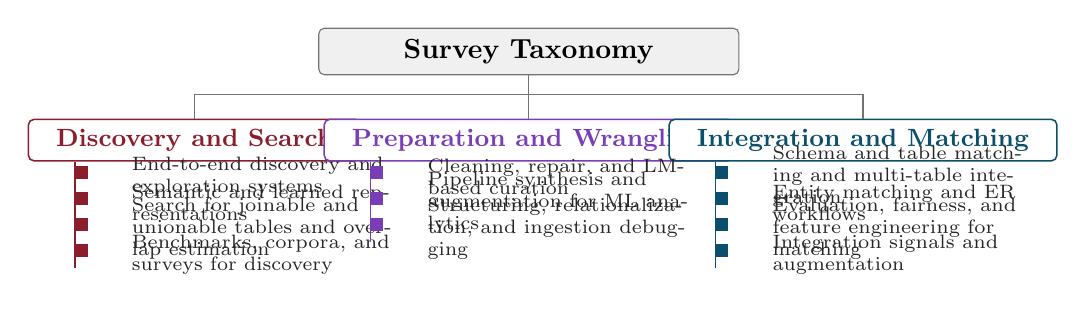
\begin{tikzpicture}[
  font=\scriptsize,
  >=Latex,
  conn/.style={draw=black!55, line width=0.45pt},
  title/.style={draw=black!55, rounded corners=2pt, fill=black!6,
                inner xsep=10pt, inner ysep=4pt, align=center,
                minimum width=0.44\textwidth},
  cat/.style={rounded corners=2pt, fill=white,
              inner xsep=10pt, inner ysep=3.5pt, align=center,
              minimum width=0.26\textwidth, line width=0.55pt},
  itemtext/.style={anchor=west, text=black!85, text width=0.27\textwidth}
]

% Colors
\definecolor{discC}{HTML}{8B1E2D}
\definecolor{prepC}{HTML}{7A3DB8}
\definecolor{inteC}{HTML}{0B4F6C}

% Bullet square size
\def\bs{1.6mm}

\def\gapTop{5.5mm}
\def\barDrop{2.4mm}
\def\stem{2.2mm}
\def\ygap{3.3mm}
\def\xoff{6.0mm}
\def\spineInset{6mm}

% --- Top title ---
\node[title] (root) {\textbf{\normalsize Survey Taxonomy}};

% --- Phase boxes ---
\node[cat, draw=discC, text=discC, below=\gapTop of root, xshift=-0.35\textwidth] (disc)
  {\textbf{\small Discovery and Search}};
\node[cat, draw=prepC, text=prepC, below=\gapTop of root] (prep)
  {\textbf{\small Preparation and Wrangling}};
\node[cat, draw=inteC, text=inteC, below=\gapTop of root, xshift= 0.35\textwidth] (inte)
  {\textbf{\small Integration and Matching}};

% --- Connector bar ---
\coordinate (barC) at ($(root.south)+(0,-\barDrop)$);
\coordinate (barL) at ($(disc.north |- barC)$);
\coordinate (barR) at ($(inte.north |- barC)$);

\draw[conn] (root.south) -- (barC);
\draw[conn] (barL) -- (barR);
\draw[conn] (barL) -- (disc.north);
\draw[conn] (barC) -- (prep.north);
\draw[conn] (barR) -- (inte.north);

% ---------- Discovery ----------
\coordinate (discStem) at ($(disc.south west)+(\spineInset,0)$);
\coordinate (discB1)   at ($(discStem)+(0,-\stem)$);
\coordinate (discB2)   at ($(discB1)+(0,-\ygap)$);
\coordinate (discB3)   at ($(discB2)+(0,-\ygap)$);
\coordinate (discB4)   at ($(discB3)+(0,-\ygap)$);

\draw[conn, draw=discC] (discStem) -- ($(discB4)+(0,-1.4mm)$);

\foreach \p/\txt in {
  discB1/{End-to-end discovery and exploration systems},
  discB2/{Semantic and learned representations},
  discB3/{Search for joinable and unionable tables and overlap estimation},
  discB4/{Benchmarks, corpora, and surveys for discovery}
}{
  \fill[discC] (\p) rectangle ++(\bs,\bs);
  \node[itemtext] at ($(\p)+(\xoff,0.3mm)$) {\txt};
}

% ---------- Preparation ----------
\coordinate (prepStem) at ($(prep.south west)+(\spineInset,0)$);
\coordinate (prepB1)   at ($(prepStem)+(0,-\stem)$);
\coordinate (prepB2)   at ($(prepB1)+(0,-\ygap)$);
\coordinate (prepB3)   at ($(prepB2)+(0,-\ygap)$);

\draw[conn, draw=prepC] (prepStem) -- ($(prepB3)+(0,-1.4mm)$);

\foreach \p/\txt in {
  prepB1/{Cleaning, repair, and LM-based curation},
  prepB2/{Pipeline synthesis and augmentation for ML analytics},
  prepB3/{Structuring, relationalization, and ingestion debugging}
}{
  \fill[prepC] (\p) rectangle ++(\bs,\bs);
  \node[itemtext] at ($(\p)+(\xoff,0.3mm)$) {\txt};
}

% ---------- Integration ----------
\coordinate (inteStem) at ($(inte.south west)+(\spineInset,0)$);
\coordinate (inteB1)   at ($(inteStem)+(0,-\stem)$);
\coordinate (inteB2)   at ($(inteB1)+(0,-\ygap)$);
\coordinate (inteB3)   at ($(inteB2)+(0,-\ygap)$);
\coordinate (inteB4)   at ($(inteB3)+(0,-\ygap)$);

\draw[conn, draw=inteC] (inteStem) -- ($(inteB4)+(0,-1.4mm)$);

\foreach \p/\txt in {
  inteB1/{Schema and table matching and multi-table integration},
  inteB2/{Entity matching and ER workflows},
  inteB3/{Evaluation, fairness, and feature engineering for matching},
  inteB4/{Integration signals and augmentation}
}{
  \fill[inteC] (\p) rectangle ++(\bs,\bs);
  \node[itemtext] at ($(\p)+(\xoff,0.3mm)$) {\txt};
}

\end{tikzpicture}
\caption{Taxonomy of data lake research from discovery and search to analytics-ready outputs via preparation and integration.}
\label{fig:taxonomy}
\end{figure*}


Figure~\ref{fig:taxonomy} shows the three classes and their categories. Together, they reflect the common path from raw lake contents to analytics-ready outputs.


\subsection{Classes and Their Categories}
\label{sec:taxonomy-classes}
Below, I define each class by its primary output and recurring tasks. The full category breakdown is shown in Figure~\ref{fig:taxonomy}.

% ----------------------
\subsubsection{Discovery and Search}
\paragraph{Output.} A ranked list of candidate data sources (tables, columns, or derived views) for the analyst to explore, join, or union.

End-to-end systems combine background work such as profiling tables and keeping indexes up to date with real-time search and interactive exploration~\cite{10.14778/3685800.3685880,11112882,10.14778/3659437.3659461}.
Representation methods learn compact vector embeddings~\cite{10.14778/3587136.3587146,11113165} or statistical sketches~\cite{11113110} for columns and tables, so that search can rely on meaning rather than exact text matches, even when metadata is missing or inconsistent.
Join search, union search, and overlap estimation find candidate tables that share data with a given seed table, then score how strongly each candidate is related. These are discovery-time steps: they identify candidates but do not produce the final merged table.
Corpora such as GitTables and benchmarks such as LakeBench~\cite{10.14778/3659437.3659448} support fair comparison and model training at lake scale.


% ----------------------
\subsubsection{Preparation and Wrangling}
\paragraph{Output.} Cleaned or transformed tables, well-structured relational views, and reusable automated workflows that can run again when new data arrives.

Cleaning methods fix errors and reduce data quality problems~\cite{10.14778/3675034.3675051}. Language-model-based curation methods~\cite{10.14778/3574245.3574258,10.14778/3611540.3611624} and transform-reuse systems~\cite{10.14778/3611540.3611628} build reusable cleaning workflows---for example, a pipeline that detects and corrects misspelled city names.
Pipeline synthesis methods~\cite{10.1145/3698831,10.1145/3588945} search for the best sequence of processing steps (such as removing duplicates, then standardizing dates, then adding a computed column) that improve results for a downstream task like training a classifier. Closely related automation methods augment features~\cite{11113027} or assemble BI models from input tables~\cite{10.14778/3603581.3603596}.
Structuring methods convert messy inputs (such as nested JSON files or inconsistent spreadsheets) into clean relational tables~\cite{10.14778/3626292.3626294,10.1145/3665252.3665269,10.14778/3681954.3682019}. Ingestion debugging methods help diagnose errors that occur when data is first loaded into the lake~\cite{10.14778/3611540.3611595}.


% ----------------------
\subsubsection{Integration and Matching}
\paragraph{Output.} Column matches, entity matches or clusters, and merged datasets.

Schema and table integration methods line up columns across multiple tables and apply explicit merge rules that determine how partial facts from different sources are combined~\cite{10.1145/3555041.3589732,10.14778/3574245.3574274,10.14778/3742728.3742757,10184612}.
ER workflows combine \emph{blocking}, \emph{matching}, and \emph{clustering}. These workflows must balance labeling cost against accuracy~\cite{10.1145/3709715,10.1145/3588722,10.1145/3588712,10.1145/3626711,10.1145/3588938}.
Evaluation work studies speed-versus-quality trade-offs in filtering~\cite{10184692}, subgroup fairness~\cite{10.14778/3611479.3611525}, and low-cost feature construction~\cite{11112979,10.14778/3681954.3681987}.
Other methods produce shared evidence---such as approximate foreign-key relationships~\cite{10.1145/3588929}, shared embeddings~\cite{10184556}, and selectively retrieved external data~\cite{10.14778/3611479.3611535,10.14778/3603581.3603602}---that can help multiple integration tasks at once.



% ==========================================================
\section{Literature Review}
% ==========================================================

% ----------------------
\subsection{Discovery and Search}
The reviewed discovery literature addresses retrieval in large lakes with weak metadata and incomplete documentation. It includes 17 counted method papers plus 2 survey/tutorial papers that I discuss for context.

The literature shows four recurring patterns. First, systems are moving from single search features to end-to-end stacks that handle indexing, search, and user interaction together. Second, retrieval quality increasingly depends on learned embeddings rather than metadata alone. Third, join search, union search, and overlap estimation serve as building blocks for later integration. Fourth, shared corpora and benchmarks are essential for fair comparison.

\subsubsection{End-to-end Discovery and Exploration Systems}
End-to-end discovery systems return ranked tables, derived views, or dataset augmentations. A common architecture has three parts: (i)~offline enrichment (profiling, indexing); (ii)~online retrieval (keyword, join, union, and view search); and (iii)~interactive exploration.

CHORUS uses a large language model (a ``foundation model'') to produce shared understanding of each table---for example, detecting what category a table belongs to, what type each column is, and which columns could be used to join tables together---and then reuses those annotations for indexing, filtering, and ranking. Because one model drives several tasks, signals can be reused efficiently, but prompt sensitivity, non-determinism, and cost can also affect multiple decisions at once. BLEND makes the discovery pipeline explicit and tunable by introducing \emph{discovery plans}---multi-step workflows written in a declarative style (the user states \emph{what} to find, not \emph{how})---that mix retrieval, composition, and ranking steps while connecting offline indexes to real-time execution. LakeCompass packages the same general idea as a single operational stack for storage, indexing, keyword search, join and union search, and interactive exploration.

Other systems specialize the user-facing side of this process. METAM~\cite{10184845} lets downstream task utility steer ranking, so candidate datasets are judged by whether they improve the target analysis rather than only by similarity or joinability. Selecting Sub-tables~\cite{10184535} makes large results easier to inspect by surfacing compact, informative previews, while Ver~\cite{10184768} handles ambiguity in \emph{view discovery} by exploring multiple join structures, pruning redundant options, and asking targeted questions to narrow down the intended merged view.

\subsubsection{Semantic and Learned Representations for Discovery}
Because meaning is rarely written down explicitly in data lakes, many methods learn compact embeddings for columns and tables so that search can compare meaning rather than exact text.

CMDL~\cite{10.14778/3611479.3611533} extends discovery beyond tables by embedding columns and unstructured documents into a shared vector space, using weak supervision to create training signal when labeled cross-modal examples are scarce. Starmie learns \emph{contextualized} column embeddings in which each column is interpreted through its table context, making semantic union search more robust than matching on isolated column text alone. LIFTus addresses heterogeneous columns such as numeric IDs and patterned strings by encoding each column through multiple \emph{aspects} and fusing them into a single retrieval representation, while TabSketchFM reduces token and cost overhead by compressing each table into a compact statistical sketch that a transformer can read directly.

\subsubsection{Join and Union Search, and Overlap Estimation}
Join search, union search, and overlap estimation are tightly connected building blocks for \emph{table enrichment}---the process of adding useful rows or columns to a starting table. Given a \emph{seed table} (the analyst's starting point), systems retrieve a small set of candidates that can be joined (linked by a shared key) or unioned (stacked because they have compatible columns), then score how strongly each candidate relates to the seed. This is still discovery: the system identifies candidates but does not yet produce a final merged table.

DeepJoin~\cite{10.14778/3603581.3603587} treats joinability as a learned retrieval problem by encoding columns with a pre-trained language model and retrieving top-$k$ join partners through approximate nearest-neighbor indexing, making search more robust to spelling and formatting variation. SANTOS~\cite{10.1145/3588689} focuses on unionability by modeling semantic relationships across columns rather than relying only on surface overlap, while Nested/Joined Lake Search~\cite{10.14778/3681954.3682005} extends the candidate space to \emph{join-nest} results built dynamically from multiple tables. Armadillo~\cite{10.1145/3725365} abstracts across join, union, and deduplication by learning graph-based embeddings whose similarity approximates table overlap at scale.

\subsubsection{Benchmarks, Corpora, and Surveys for Discovery}
Discovery at lake scale depends on shared resources---corpora for training, benchmarks for fair comparison, and indexing techniques for efficient search.

Rottnest~\cite{11113229} addresses the operational side of discovery by proposing a lakehouse indexing protocol that manages index-building and update overhead in evolving storage. GitTables~\cite{10.1145/3588710} supplies a large relational-style corpus with semantic-type annotations for representation learning and table-understanding tasks, and LakeBench provides labeled workloads for join and union discovery so systems can be compared on both quality and runtime. The two survey papers complement these resources from different angles: the Data Discovery Survey emphasizes operational concerns such as mismatched evaluation setups and weak reporting of computational cost, while the Table Discovery Survey consolidates methods and open problems around robustness and efficiency.

Once candidate data sources are surfaced, the next phase focuses on transforming these often-messy results into clean, well-structured inputs that can be used for analytics and downstream integration.


% ----------------------
\subsection{Preparation and Wrangling}
% ----------------------

The reviewed preparation literature emphasizes turning discovered candidates into stable inputs for analysis. The main idea is \emph{repeatable automated workflows} instead of one-time manual fixes. Because discovery often retrieves messy data and integration assumes reasonably well-structured inputs, preparation directly affects how well later matching works. If preparation fails to standardize date formats, for example, integration may incorrectly treat matching dates as different values---an impact easy to miss when evaluation only reports local metrics.



\subsubsection{Cleaning, Repair, and LM-based Curation}
Data lakes make classic data-quality problems worse: errors are frequent and come in many forms, and the context needed to understand dirty values is often unavailable. Methods in this category focus on two goals: (i)~\emph{deployable repair} that actually reduces the number of errors in a table, and (ii)~\emph{reusable curation workflows} that turn cleaning logic into automated, controllable steps.

Different preparation methods optimize different goals---consistency, net error reduction, or downstream model accuracy---and the automatic data repair study~\cite{10.14778/3675034.3675051} shows why mixing these goals without stating them clearly can be misleading.

Automatic Data Repair argues that repair methods should be evaluated by whether they reduce the total number of errors, not just by how many cells they change, and benchmarks methods across datasets and error types while proposing safeguards against \emph{incorrect repairs}. Foundation Models for Data Tasks~\cite{10.14778/3574245.3574258} recasts traditional preparation tasks as prompts to large language models, showing broad task coverage but also surfacing privacy concerns and failures on domain-specific conventions. Lingua Manga turns that idea into reusable curation pipelines through modular templates and a small scripting language that reduces expensive model calls and supports rerunnable workflows as new lake data arrives, while DataRinse reaches similar reuse goals without language models by mining semantic transformation patterns from existing preparation code and presenting them as coherent human-in-the-loop recommendations.



\subsubsection{Pipeline Synthesis and Augmentation for ML Analytics}
Pipeline synthesis treats data preparation as a search problem: given raw tables and a goal (such as training an accurate classifier), the system automatically finds the best sequence of processing steps---cleaning, transforming, and adding features---that improves the final result within a given budget.

CtxPipe addresses the huge search space of possible processing sequences by using dataset characteristics and task feedback to prioritize transformations that are more likely to improve the downstream model. HAIPipe~\cite{10.1145/3588945} keeps that search grounded in expert intent by starting from a human-written pipeline and augmenting it automatically, while Featpilot~\cite{11113027} treats augmentation as join-path search over other lake tables so that useful features can be added through multi-hop joins. Auto-BI~\cite{10.14778/3603581.3603596} pushes the same idea toward business-intelligence outputs by discovering the \emph{join model} needed to connect multiple tables for dashboards and reports.



\subsubsection{Structuring, Relationalization, and Ingestion Debugging}
This category covers two related problems: (1)~converting messy lake inputs (such as nested JSON files, HTML tables, or unstructured documents) into clean, queryable relational tables (standard row-and-column format), and (2)~detecting and fixing errors that occur during \emph{ingestion}---the process of loading data into the lake.

Evaporate~\cite{10.14778/3626292.3626294} builds queryable tables from unstructured documents by either extracting values with a language model or synthesizing extraction code, and can combine multiple synthesized extractors with weak supervision to improve coverage. Auto-Tables~\cite{10.1145/3665252.3665269} tackles irregular spreadsheet layouts by synthesizing multi-step relationalization programs without input--output examples, while ReCG~\cite{10.14778/3681954.3682019} induces usable schemas from semi-structured collections by clustering records, generalizing clusters into schema fragments, and merging them into a compact global schema. On the debugging side, CM Explorer isolates ingestion failures through conditional data tests over targeted subsets rather than only global statistics, and XDBC~\cite{10.1145/3725294} treats cross-system data movement itself as a configurable transfer pipeline whose stages can be auto-tuned for throughput.


% ----------------------
\subsection{Integration and Matching}

The reviewed integration literature organizes around four concerns: (i)~schema-level alignment and merge rules, (ii)~entity resolution as a multi-step workflow, (iii)~fairness-aware evaluation, and (iv)~reusable integration signals such as approximate foreign-key relationships or learned embeddings. Here, an approximate foreign-key relationship is a noisy join hint: values in one column often correspond to values in another even when formatting differences or typos prevent exact matches. A broader trend is that integration outputs increasingly feed back into discovery and preparation as reusable evidence.


\subsubsection{Schema and Table Matching and Integration}
\label{sec:lit-sm-integration}

Schema matching and table integration form the core of the alignment process. Given a set of candidate tables found during discovery, systems must determine which columns correspond to each other, then apply merge rules to combine everything into one analysis-ready table. This is different from join or union search in the discovery phase: here the system actually performs the merge and produces a final output.

\paragraph{End-to-end integration pipelines.}
DIALITE treats integration as a complete workflow: first \emph{discover} relevant tables, then \emph{align and integrate} them by matching columns and merging rows, and finally \emph{analyze} the merged table. Different discovery methods can feed into the same alignment stage, and intermediate outputs (candidate set, column alignments, merged table) can be inspected at each step.

\paragraph{Integration semantics and operators.}
ALITE argues that integration quality depends on clear merge rules, often called \emph{integration semantics}, not just pairwise joins. For example, when one table has a customer's phone number but not their email, and another table has the email but not the phone number, the merge rule should combine both pieces of information into one row. ALITE first performs global column matching by assigning shared IDs to matched columns, then applies \emph{Full Disjunction}---a merge strategy designed for tables with many missing values and partial overlaps. It breaks this into reusable operators: outer union, subsumption, and complementation.

The core idea, also central in DIALITE, is to connect partial facts across sources rather than just running local joins. Discovery finds the tables; the harder step is deciding exactly how to combine them so the final output is complete and useful.

\paragraph{LM-powered schema matching.}
Magneto uses a two-stage design: a smaller, cheaper language model first proposes and ranks candidate column matches, and then a larger, more powerful model validates the hard cases for higher precision. PLM Schema Matching targets enterprise settings where access to actual data is limited (for privacy reasons) and the target schema is large and domain-specific. It adapts pre-trained language models with minimal labeled examples to reduce the effort needed from human experts.


\subsubsection{Entity Matching and ER Workflows}

This literature treats ER as a workflow rather than a single classifier.

\paragraph{Progressive and intent-aware matching.}
Progressive EM studies pay-as-you-go ER: when time or budget is limited, the system prioritizes the most valuable comparisons first. It breaks the process into filtering, weighting, scheduling, and matching steps. FlexER shows that what counts as a ``match'' can depend on downstream intent: the same two product listings may be treated as equivalent for one task and distinct for another. It models those multiple valid decisions as multi-label classification.

\paragraph{Lowering supervision cost and unifying models.}
Obtaining labeled training data for EM is expensive. WeakSup GT Inference addresses this by combining noisy weak-supervision signals with a label model that enforces global constraints such as transitivity. Battleship targets low-resource settings with active learning that strategically selects the most informative record pairs for a human to label. Unicorn unifies multiple matching tasks into a single shared model with task-specific output heads.


\subsubsection{Evaluation, Fairness, and Feature Engineering for Matching}

Recent EM work treats matching as a configurable pipeline where blocking strategies, fairness across demographic groups, and feature engineering all matter.

\paragraph{Benchmarking filtering under quality--runtime targets.}
Filtering Benchmarks compares different blocking strategies (for example, rule-based blocking versus approximate nearest-neighbor retrieval) for candidate-pair generation. It shows that fair comparisons require careful tuning of many interacting parameters, and reports effectiveness alongside running time and scalability.

\paragraph{Fairness-aware evaluation for EM}
Fairness Lens audits EM methods across demographic subgroups---for example, checking whether matching accuracy differs between common names and uncommon names, or between majority and minority groups. It shows that overall accuracy can look good while hiding significant disparities for specific subgroups, and advocates for fairness-sensitive metrics that go beyond population-level averages.

\paragraph{Practical feature selection and attribute enrichment.}
DescSim Rules mines interpretable similarity rules by analyzing column descriptions and value distributions, allowing expensive model retraining to be done offline. Relation Enrichment improves matching by adding a small set of carefully chosen auxiliary attributes from related tables---for example, adding a customer's city to help disambiguate customers with the same name.


\subsubsection{Integration Signals and Augmentation}
\label{sec:integration-signals}

This category covers methods that output approximate foreign-key relationships, shared embeddings, or targeted augmentation results rather than a final merged table.

\paragraph{Relaxed dependency signals for noisy join discovery.}
SIND introduces \emph{similarity inclusion dependencies} (sINDs). In a clean database, a foreign-key relationship means every value in one column appears exactly in another. In noisy data lakes, exact containment rarely holds, so sINDs allow sufficiently similar values instead. That makes them useful as approximate foreign-key hints for join discovery and integration.

\paragraph{Reusable representation signals across tasks.}
Sudowoodo pre-trains similarity-aware embeddings using contrastive learning on unlabeled data. These embeddings can then be reused across multiple integration tasks, reducing the need for labeled training data.

\paragraph{On-demand external enrichment via progressive querying.}
Entity Augmentation studies how to enrich lake entities using external sources that are only accessible through keyword-search interfaces (such as web APIs). It proposes a progressive, feedback-driven querying strategy: submit initial queries, check which results are useful, and refine subsequent queries based on what was found.

\paragraph{Analysis-driven augmentation for causal validity.}
Causal DI addresses a specific analytics need: ensuring that integrated data supports valid causal analysis. It looks for missing \emph{confounders}, meaning variables that influence both the treatment and the outcome, retrieves them from external sources, and then builds a causal graph to decide which variables should be integrated.


\label{sec:pubs-by-phase}


% ==========================================================
\section{Discussions and Challenges}
\label{sec:discussion-challenges}
% ==========================================================

This section presents the main lessons from the survey and the open problems that remain.

\subsection{Phases Are Connected but Evaluation Is Isolated}
Most methods report metrics for only one phase, which can hide downstream problems. A discovery method with high precision may still retrieve tables that are hard to integrate. A practical lesson is to report stage-level results, maintenance cost, and at least one end-to-end outcome together.

Methods in different phases also optimize different goals---ranking quality, format consistency, or match accuracy---and without naming these differences, cross-method comparisons can look cleaner than they actually are.

\subsection{Ambiguity and User Intent}
In data lakes, metadata is often missing or vague, and the same query can have many plausible answers. For example, searching for ``customer data'' might return sales records, support tickets, or demographic profiles---all valid depending on the analyst's goal. Discovery systems address this by supporting interactive refinement rather than assuming a single correct answer. On the integration side, the same pair of records can be considered a ``match'' or ``non-match'' depending on the downstream task, as FlexER illustrates with intent-aware entity resolution. This challenges the single-ground-truth assumption built into many benchmarks. An important open problem is \emph{intent-conditioned evaluation}: explicitly varying the analyst's goal and reporting how robust each method is across different intents and domains.

\subsection{Scalability, Cost, and Maintenance}
At the scale of real data lakes (thousands to millions of tables), major costs come from infrastructure: generating embeddings for every column, building and maintaining search indexes, and keeping everything up to date as new data arrives. End-to-end systems, benchmarks, and operations surveys all show why cost should be reported alongside effectiveness. Preparation and integration face similar pressures: pipeline synthesis requires repeated execution, progressive ER uses filtering and scheduling to control cost on a pay-as-you-go basis, and filtering benchmarks quantify the trade-off. Most current evaluations assume that the data does not change over time, which hides the real challenge of keeping results up to date as lake contents evolve. A key research direction is incremental maintenance---updating indexes, embeddings, and validation tests efficiently when new data arrives, rather than rebuilding everything from scratch.

\subsection{Preparation Needs Safety Checks}
Preparation can improve downstream quality, but improvements are not guaranteed. A repair system might over-edit or introduce plausible but incorrect values. Evaluation should therefore prioritize net error reduction and avoid changes that introduce more errors than they fix. Language-model-based curation adds further risks: models can hallucinate, give different answers on repeated runs, and expose private data if data is sent to an external API. Structuring methods also show that converting messy lake inputs into clean tables often requires multiple transformation steps, not just one. In practice, systems need lightweight verification hooks such as automated tests, constraint checks, and sample-based audits that can trigger a rollback or request human review when confidence is low.

\subsection{Integration Design Choices}
Integration in data lakes is not as simple as ``match columns, then join.'' Real-world tables overlap only partially and have many missing values. Merge rules must therefore preserve partial facts while combining as much evidence as possible. Full Disjunction-style approaches show that careful merge operators can significantly outperform naive pairwise joins. At the entity level, workflow-oriented ER shows that the choice of blocking and scheduling strategy and supervision strategy often matters more for end-to-end performance and cost than the choice of matching model alone. Unified matching models address part of this design space. Language-model-based matchers can reduce the need for labeled data and handle diverse formats, but they raise concerns about the reliability of model confidence scores, latency, and privacy. A key open issue is choosing merge rules and workflow steps that align with the analyst's actual goal, and evaluating those trade-offs directly.

\subsection{Fairness, Privacy, and Governance}
As lake pipelines become more automated, responsible operation becomes part of system design, not an afterthought. Fairness-aware evaluation shows that overall accuracy can mask unequal error rates across groups---for example, an entity-matching system may work well for common names but poorly for uncommon ones. Language-model-based data tasks also raise privacy risks: converting data into text prompts and sending them to an external API can leak sensitive information or violate organizational policies. Governance rules---organizational policies about which tables can be joined, which attributes can be exposed, and which external sources can be used---should be built into the pipeline as planning constraints, not checked only after the fact. Open problems include auditing fairness at every stage (not just the final matcher), developing privacy-preserving indexing and language-model techniques, and building integration planners that respect organizational policies by design.

\subsection{Benchmark Gaps and Shared Test Collections}
Shared corpora and benchmarks have improved comparability within each phase: GitTables and LakeBench standardize parts of discovery evaluation, and ER benchmarks support workflow comparison. Learned embeddings and profiling signals are also reused across tasks. However, few resources cover the full pipeline---discovery through preparation through integration---under realistic conditions such as data updates, changing analyst intent, and explicit cost reporting. A concrete next step is a pipeline test collection that combines workloads from all three phases, provides ground truth at each stage, and tracks computational cost.

Such a test collection is especially useful because failures often occur at the boundaries between phases---for example, discovery returning structurally incompatible tables, or preparation removing values needed for later matching.

\subsection{Threats to Validity}
This study has limits. I searched three venues (SIGMOD, PVLDB, ICDE), so methods published elsewhere may be missing. Some methods could fit more than one category, so any taxonomy compresses real overlap. The chosen time window keeps the survey focused on recent work, but it excludes methods outside that window. Methods across phases optimize different goals such as ranking quality, consistency, and match accuracy, so side-by-side comparison is inherently imperfect. Limited code and data release makes full reproducibility difficult. I keep phase-specific metrics separate and note where reproducibility is weak.

% ==========================================================
\section{Conclusion}
% ==========================================================
I reviewed recent work across discovery, preparation, and integration. Discovery increasingly combines learned representations with scalable indexing and retrieval; preparation increasingly produces repeatable automated workflows but still needs safety checks; and integration increasingly depends on workflow design and analyst intent rather than a single matching score. A natural next step is stronger end-to-end evaluation under realistic conditions including data updates, ambiguous intent, and explicit cost measurement.


% ==========================================================
\balance
\bibliographystyle{ACM-Reference-Format}
\bibliography{ref}
% ==========================================================

\end{document}
